%% This tex file reads files.lst and generates the pdf from the files listed
%% in there, don't run this directly instead run the Makefile


\documentclass{article}
\usepackage[landscape,twocolumn,nomarginpar,height=7in,width=10in,top=1in,bottom=0.5in,columnsep=0.5in]{geometry}
\usepackage[T1]{fontenc}
\usepackage{fancyvrb}
\usepackage{fancyhdr}
\usepackage{listings}
\usepackage{caption}
\usepackage{color}
\usepackage{pdfpages}
\pagestyle{fancy}
\lhead[University of Wisconsin - Madison]{University of Wisconsin - Madison}
\rhead[\thepage]{\thepage}
\lfoot[]{}
\cfoot[]{}
\rfoot[]{}

\def\cleanws#1 {#1}
\def\stripslash#1#2\ssend{#2}
\def\makesane[#1]{\expandafter\expandafter\expandafter\stripslash\expandafter\string\csname#1\endcsname\ssend}

\lstloadlanguages{[GNU]C++,Java}
\lstset{
basicstyle=\fontsize{7pt}{8.1pt}\ttfamily,
keywordstyle=\color{blue}\bfseries,
language=[GNU]C++,
columns=fixed,
numbers=left,numberstyle=\tiny,
linewidth=5in,
breaklines=true,
basewidth={0.55em,0.4em},
frame=lines,
}
\renewcommand\listfigurename{Entries}
\begin{document}
\lstlistoflistings
\newread\fstream
\openin\fstream=files.lst
\loop
\def\test{a}
\ifeof\fstream
\def\test{\relax}
\fi
\if a\test
\read\fstream to \fname
\if\fname\par
\relax
\else
\edef\fname{\expandafter\cleanws\fname}
\edef\fname{\makesane[\fname]}
\edef\fname{\noexpand\detokenize{\fname}}
\lstinputlisting[caption={[\noexpand\noexpand\noexpand\detokenize{\fname}]},title={\fname},name=\fname]{\fname}
\fi
\repeat

\onecolumn
{\center 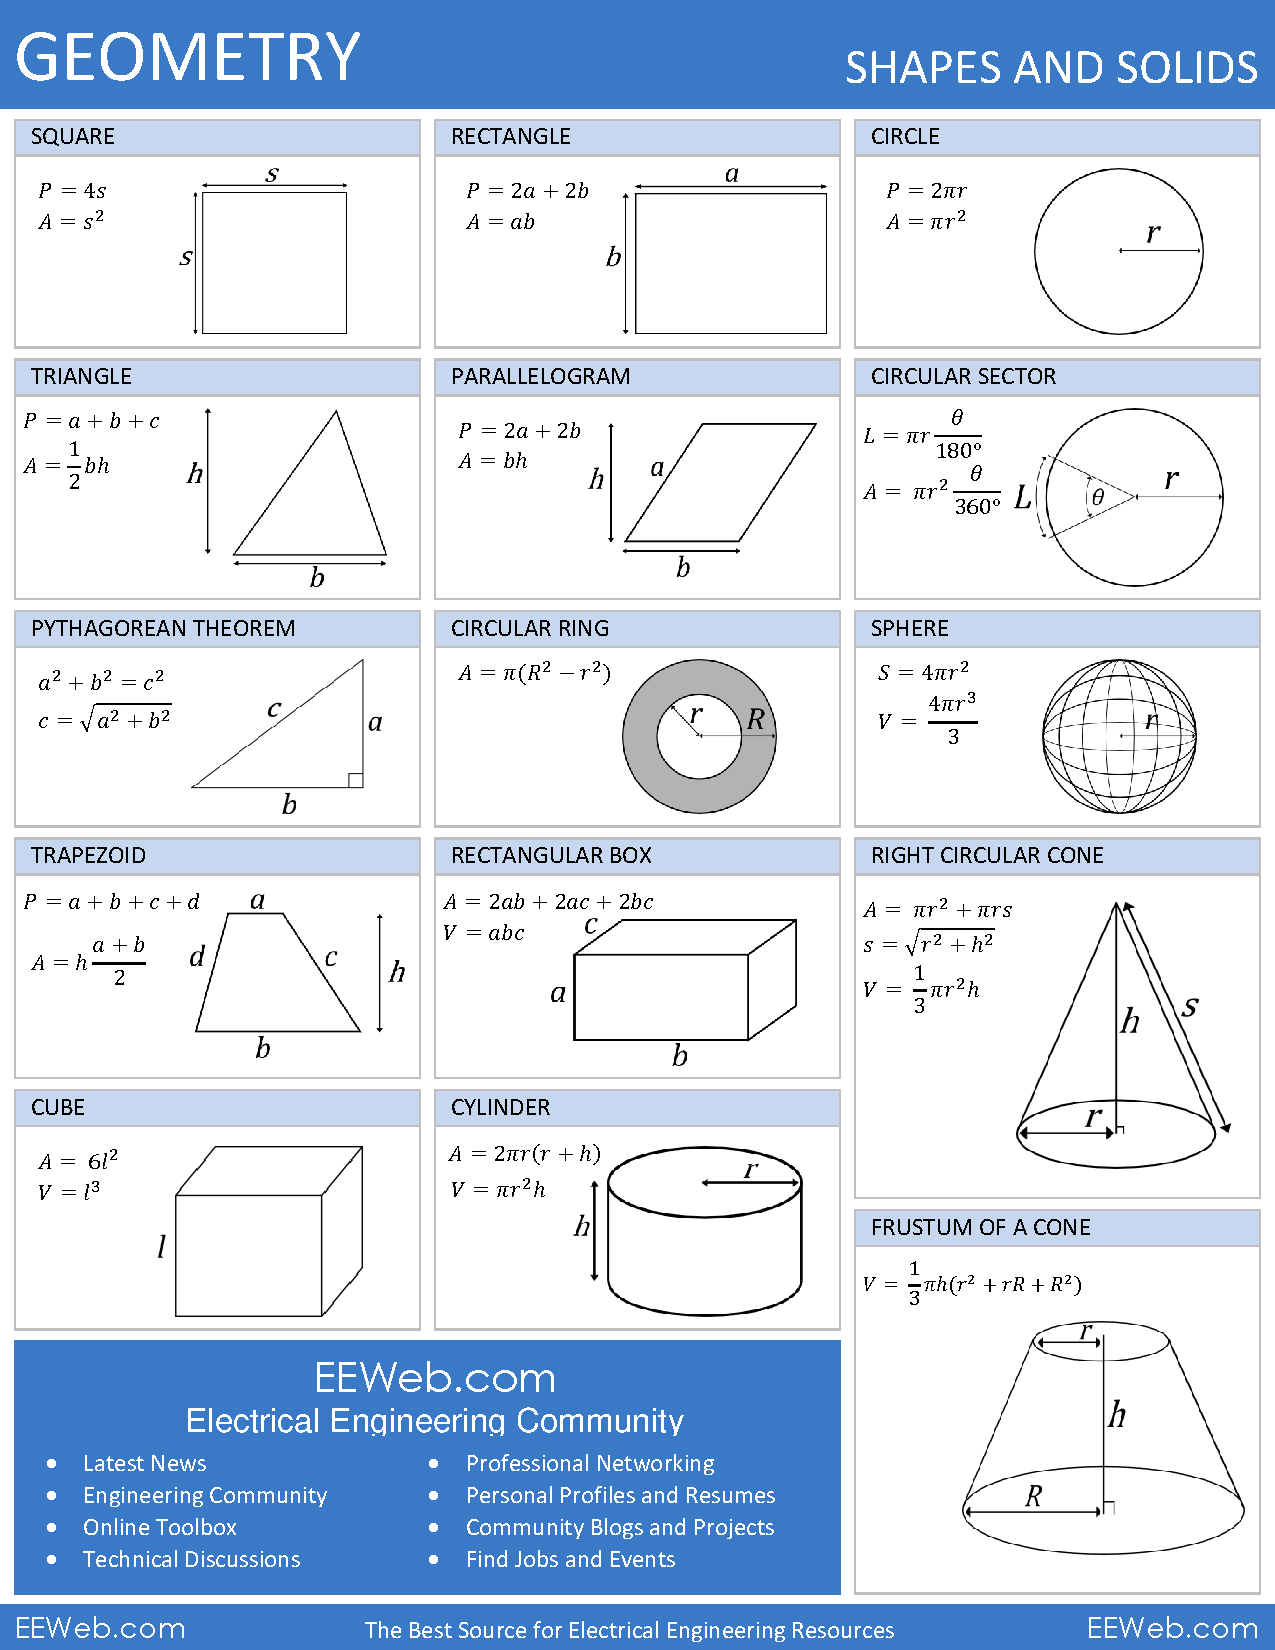
\includegraphics[angle=270,scale=.82]{geom_cheatsheet.pdf}}

\end{document}
